\documentclass[../../syllabus_1.tex]{subfiles}
\begin{document}

\chapter{Diviseurs et multiples}

\section*{Matières}
\begin{enumerate}[label=\textbf{\arabic*.}]
      \item Caractères de divisibilité.
      \item Les diviseurs.
      \item Les puissances.
      \item Nombres premiers et nombres carrés.
      \item La décomposition en facteurs premiers.
      \item Les multiples d’un nombre.
\end{enumerate}

\section{L'histoire du "TikTok Challenge" le plus cher du monde}
Lucas, un élève de 12 ans pas très fan des devoirs, supplie son père de lui donner de l'argent de poche pour s'acheter la dernière console de jeux.
Son père, qui adore les défis et les mathématiques, lui sourit et lui dit : "D'accord Lucas. Je te propose un marché pour tout le mois de juin (qui dure 30 jours) :  je te donne 1 centime aujourd'hui. Demain, je double cette somme et je te donne 2 centimes. 
Le troisième jour, je double encore et je te donne 4 centimes. 
Chaque jour, je te donne le double du jour précédent jusqu'au 30e jour."

Lucas, qui calcule très vite dans sa tête, se dit : "1 centime, puis 2, puis 4, puis 8... Au bout de dix jours, ça va faire à peine quelques pièces de monnaie. Mon père est complètement radin, il essaie de m'arnaquer !"

Lucas accepte le défi en ricanant, persuadé qu'il va devoir s'acheter une console d'occasion.

Ce qui s'est réellement passé :
\begin{itemize}[label=$\bullet$]
      \item Le jour 1 : Lucas reçoit 1 centime ($2^0$).
      \item Le jour 2 : Il reçoit 2 centimes ($2^1$).
      \item Le jour 5 : Il reçoit 16 centimes ($2^2$). 
      \item Le jour 10 : Il reçoit 512 centimes, soit 5,12 € ($2^9$). Lucas commence à s'ennuyer.
      \item Le jour 15 : Le montant continue de grandir \dots Lucas reçoit 163,84 €. Il commence à regarder les prix des consoles neuves avec un grand sourire.
      \item Le jour 20 : C'est le choc. Son père doit lui donner 5242,88 € ($2^{19}$). Son père commence à transpirer et ne rigole plus du tout.
      \item Le jour 30 (le grand final) : Pour ce seul et unique jour, son père doit verser à Lucas la somme de 5 368 709,12 € ($2^{29}$).
\end{itemize}

Le 30e jour, Lucas tend la main. Son père arrive dans la chambre avec une feuille de calcul et lui dit textuellement : "Fiston, j'ai dû vendre la maison, la voiture et je crois que je te dois aussi ton poids en lingots d'or." 
Pour la seule journée du jour 30, le père devait à Lucas 5 368 709,12 € ! Si on additionne tous les jours précédents, Lucas se retrouve à la fin du mois avec plus de 10 millions d'euros.

La morale de l'histoire : ne sous-estimez jamais un petit nombre qui a "le bras long" (un exposant). La multiplication répétée ne grandit pas sagement comme une addition, elle explose !

\newpage
\section{Rappel des caractères de divisibilité}

Les caractères de divisibilité permettent de reconnaitre si un nombre est divisible par un autre sans devoir effectuer la division.

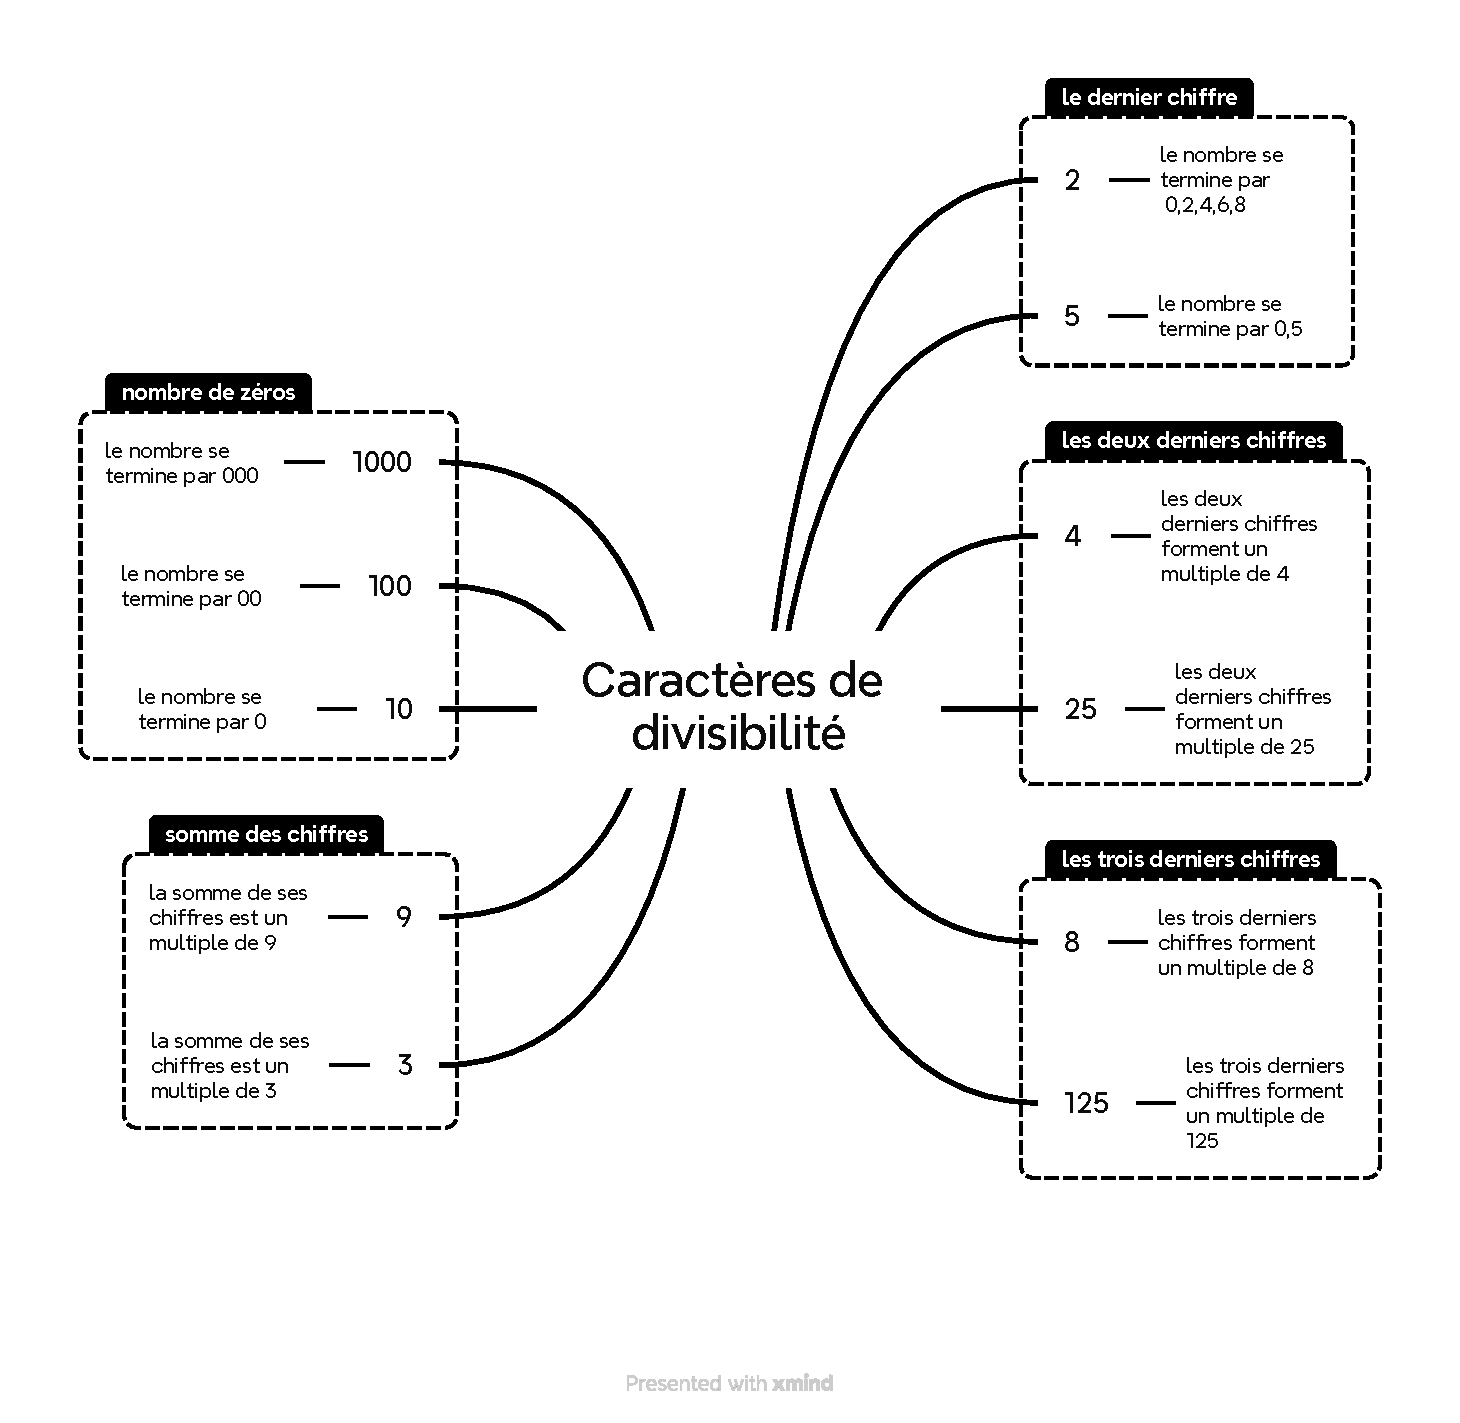
\includegraphics[width=1\linewidth]{figures/caracteres_de_divisibilite.pdf}

\newpage

\begin{exercise}
      Réponds en justifiant.
      \begin{enumerate}[itemsep=1cm, after=\vspace*{1cm}]
            \item \num{52035} est-il divisible par 5 ?
            \item \num{1000003} est-il divisible par 3 ?
            \item \num{819} est-il divisible par 9 ?
            \item \num{35150} est-il divisible par 25 ?
            \item \num{5014} est-il divisible par 4 ?
      \end{enumerate}
\end{exercise}

\begin{exercise}
      En utilisant les chiffres \numlist{3;8;9;1;6} une seule fois chacun, forme, si possible
      \begin{enumerate}
            \item le plus petit nombre naturel multiple de 3 :
            \item le plus grand nombre naturel divisible par 8 :
            \item le plus petit nombre naturel multiple de 5 :
            \item le plus petit nombre naturel divisible par 2 et par 3 :
            \item le plus grand nombre divisible par 6, mais pas par 2 :
      \end{enumerate}
\end{exercise}

\begin{exercise}
      % les options pour \num permettent d'avoir du gras.
      Complète le tableau ci-dessous en cochant d'une croix les cases pour lesquelles les divisions sont vérifiées.
      \begin{center}
            \begin{tblr}{
                        hlines,
                        vlines,
                        colspec={l*{8}{X[c]}},
                        rows={.7cm, m},
                        row{1}={gray!40, font=\bfseries},
                        column{1}={gray!40, font=\bfseries},
                        cell{1}{1}={white},
                        vline{1}={1}{white},
                        hline{1}={1}{white}
                  }
                                                                                 & 2 & 3 & 4 & 5 & 8 & 9 & 25 & 125 \\
                  560                                                            &   &   &   &   &   &   &    &     \\
                  750                                                            &   &   &   &   &   &   &    &     \\
                  \num[text-family-to-math=true, text-series-to-math=true]{1125} &   &   &   &   &   &   &    &     \\
                  \num[text-family-to-math=true, text-series-to-math=true]{3072} &   &   &   &   &   &   &    &     \\
            \end{tblr}
      \end{center}
\end{exercise}

\begin{exercise}
      \(236\) athlètes peuvent-ils défiler en rangs de 3 de front ? Justifie.
\end{exercise}

\newpage
\begin{exercise}
      Par quel(s) chiffre(s) peut-on remplacer le symbole ($\bullet$) pour que les nombres ci-dessous soient divisibles par le nombre demandé ?
      \begin{enumerate}[itemsep=1em]
            \item \(26\bullet 4\) est divisible par \(4\) si  $\bullet=$
            \item \(73\bullet 6\) est divisible par \(3\) si  $\bullet=$
            \item \(74\bullet 2\) est divisible par \(5\) si  $\bullet=$
            \item \(17\bullet 7\) est divisible par \(9\) si  $\bullet=$
            \item \(2861\bullet \) est divisible par \(6\) si  $\bullet=$
      \end{enumerate}
\end{exercise}

\section{Puissance d'un nombre}

\textbf{Première approche}

Deux élèves ont vu une des questions de l'examen de français. Ils décident de la partager chacun avec leurs deux meilleurs amis. Ceux-ci font la même chose avec leurs deux meilleurs amis. 

Combien de personnes ont-elles été mises au courant au total ? \dotsforanswer{1}
Comment peux-tu représenter ce nombre sous forme d'une puissance ? \dotsforanswer{1}

\textbf{Deuxième approche}

Une fleur de tournesol peut produire environ 100 graines. Si on replante toutes les graines, combien de plantes aura-t-on : 
\begin{itemize}[label=$\bullet$]
      \item à la première génération : \dotsforanswer{1}
      \item à la deuxième génération : \dotsforanswer{1}
      \item à la troisième génération : \dotsforanswer{1}
\end{itemize}

Les puissances de 10 sont utiles pour écrire les grands nombres. Prenons l'exemple du système métrique :
\begin{itemize}[label=$\bullet$]
      \item 1 mètre - \dotsforanswer{1}
      \item 1 décamètre - \dotsforanswer{1}
      \item 1 hectomètre - \dotsforanswer{1}
      \item 1 kilomètre - \dotsforanswer{1}
      \item 1 mégamètre - \dotsforanswer{1}
      \item 1 gigamètre - \dotsforanswer{1}
\end{itemize}

Les préfixes kilo, méga et giga sont beaucoup utilisés pour représenter de grandes quantités, notamment en informatique.
Imagine que tu as un smartphone de 128 Go (gigaoctets) et que tu souhaites le remplir avec des fichiers de 20 Mo (mégaoctets). Combien de fichiers peux-tu stocker ?
\vspace{2cm}

Une \textbf{puissance} est un produit de facteurs identiques, qui s'écrit sous la forme d'une \textbf{base} et d'un \textbf{exposant}. 

Exemple : \(2 \cdot 2 \cdot 2 \cdot 2 \) est un produit de 4 facteurs égaux (2). Il s'écrit sous forme de puissance : 
\vspace{1cm}

$3^2$ peut s'exprimer comme "3 au carré". C'est l'aire d'un carré de 3 cm de côté.

$3^3$ peut s'exprimer comme "3 au cube". C'est le volume d'un cube de 3 cm de côté.

Remarque : $4^1 = 1$ et $4^0 = 0$.

\begin{exercise}
      Écris les énoncés suivants sous la forme d'une multiplication ou d'une puissance (si possible).
      \begin{enumerate} [cols=2, itemsep=1cm]
            \item \(5 + 5 + 5 = \)
            \item \(5 \cdot 5 \cdot 5 \cdot 5 \)
            \item Le double de 6.
            \item Le cube de 5.
            \item \(7 + 7 + 7 + 7 + 7 = \)
            \item \(8 \cdot 8 \cdot 8 \cdot 8 \cdot 8 \cdot 8 = \)
            \item Le triple de 10.
            \item Le carré de 7.
      \end{enumerate}
\end{exercise}

\begin{exercise}
      Calcule les puissances suivantes.
      \begin{enumerate} [cols=2, itemsep=1cm]
            \item $2^2$=
            \item $4^2$=
            \item $3^3$=
            \item $4^3$=
            \item $8^2$=
            \item $5^3$=
      \end{enumerate}
\end{exercise}

\section{Découverte des diviseurs}

Représente dans le quadrillage ci-dessous l'ensemble des rectangles possédant exactement 24 petits carrés.
\begin{center}
      
\begin{tikzpicture}[scale=0.5]
            % grille 12 x 30
            % pour la taille de la grille : ultra thin, very thin, thin, thick, ...
            \draw[color=gray!70, thick] (0,0) grid (30,10);
      \end{tikzpicture}
\end{center}

Dimensions possibles de chaque rectangle : \dotsforanswer{1}

Fais de même avec 26 petits carrés.
\begin{center}
      
\begin{tikzpicture}[scale=0.5]
            % grille 12 x 30
            \draw [color=gray!70, thick] (0,0) grid (30,10);
      \end{tikzpicture}
\end{center}

Dimensions possibles de chaque rectangle : \dotsforanswer{1}

\newpage
\begin{exercise}
      % on utilise la notation a X b pour les dimensions
      Quelles sont les dimensions possibles d'un rectangle constitué du nombre de carrés ci-dessous.
      \begin{enumerate}[itemsep=1em]
            \item 8 carrés ?
            \item 15 carrés ?
            \item 50 carrés ?
            \item 48 carrés ?
      \end{enumerate}
\end{exercise}

\medbreak
Que représentent ces dimensions par rapport aux nombres de carrés ?
\dotsforanswer{2}

\vfill

\begin{exercise}
      Détermine les éléments des ensembles ci-dessous.
      \begin{enumerate}[cols=2, itemsep=3em]
            \item \(div~9 = \)
            \item \(div~7 = \)
            \item \(div~100 = \)
            \item \(div~1 = \)
            \item \(div~12 = \)
      \end{enumerate}
\end{exercise}

\begin{exercise}
      Vrai ou faux ?
      \begin{enumerate}[itemsep=1cm]
            \item Plus un nombre naturel est grand, plus il admet de diviseurs.
            \item 1 divise tous les nombres.
      \end{enumerate}
\end{exercise}

\newpage
\section{Nombres particuliers}

\subsection{Nombres carrés}
Dans le quadrillage ci-dessous, trace en bleu tous les rectangles constitués de 16 carrés.
\begin{center}
      
\begin{tikzpicture}[scale=0.5]
            % grille 12 x 30
            % pour la taille de la grille : ultra thin, very thin, thin, thick, ...
            \draw[color=gray!70, thick] (0,0) grid (30,10);
      \end{tikzpicture}
\end{center}
Que remarques-tu ? \dotsforanswer{2}
% Le nombre 16 peut être représenté par un carré. On l'appelle donc un "nombre carré"

Ce nombre possède un nombre impair de diviseurs car lorsque tu le décompose en différents produits,
l'un d'eux possèdera deux facteurs identiques.
\begin{align*}
      1 \cdot 16        & = 16  \\
      2 \cdot 8         & = 16  \\
      \Aboxed{4 \cdot 4 & = 16}
\end{align*}
On trouvera donc que les $div~16=\big\lbrace 1,2,4,8,16 \big\rbrace$.

Géométriquement, les nombres carrés font référence à l'aire d'un carré.

\begin{exercise}
      Pour les nombres carrés ci-dessous, es-tu capable de retrouver la longueur du côté du carré ?
      \begin{enumerate}[cols=3]
            \item
                  \begin{tikzpicture}[baseline=(current bounding box.west)]
                        \draw (0,0) rectangle (2,2)node[midway]{$9$};
                        \draw (current bounding box.south)node[below=1em]{\dots};
                  \end{tikzpicture}
            \item
                  \begin{tikzpicture}[baseline=(current bounding box.west)]
                        \draw (0,0) rectangle (2,2)node[midway]{$25$};
                        \draw (current bounding box.south)node[below=1em]{\dots};
                  \end{tikzpicture}
            \item
                  \begin{tikzpicture}[baseline=(current bounding box.west)]
                        \draw (0,0) rectangle (2,2)node[midway]{$100$};
                        \draw (current bounding box.south)node[below=1em]{\dots};
                  \end{tikzpicture}
      \end{enumerate}
\end{exercise}

\newpage
\begin{exercise}
      Complète le tableau ci-dessous pour trouver les dix premiers nombres carrés.
      \begin{center}
            \begin{tblr}{
                        hlines,
                        vlines,
                        columns = {c, 0.045\linewidth},
                        column{1} = {2cm, gray!40, font=\bfseries},
                        rows = {.7cm, m}}
                  Longueur du côté &  &  &  &  &  &  &  &  &  &  &  & $n$ \\
                  Aire du carré    &  &  &  &  &  &  &  &  &  &  &  &     \\
            \end{tblr}
      \end{center}
\end{exercise}

\subsection{Nombres premiers}

Dans le quadrillage ci-dessous, trace en bleu tous les rectangles constitués de 13 carrés, et en vert tous les rectangles constitués de 7 carrés.
\begin{center}
      
\begin{tikzpicture}[scale=0.5]
            % grille 12 x 30
            % pour la taille de la grille : ultra thin, very thin, thin, thick, ...
            \draw[color=gray!70, thick] (0,0) grid (30,10);
      \end{tikzpicture}
\end{center}
\dotsforanswer{3}[Que remarques-tu ?]
\dotsforanswer{2}[Un nombre premier est]

Les nombres premiers à retenir (crible d'Hératostène pour les nombres premiers inférieurs à 100) : 

\newpage
\begin{exercise}
      Vrai ou faux ? Justifie dans les deux cas.
      \begin{enumerate}[itemsep=1cm, after=\vspace*{1cm}]
            \item 1 est un nombre premier.
            \item Tous les nombres impairs sont des nombres premiers.
            \item La différence entre deux nombres premiers vaut toujours deux.
            \item Il n'existe aucun nombre premier qui soit pair.
            \item Il n'existe pas de nombres premiers consécutifs.
      \end{enumerate}
\end{exercise}

\begin{exercise}
      Josette affirme à son petit frère : \og Il n'existe aucun nombre premier qui termine par 5 \fg{}. Est-ce vrai ? Explique.
      \vspace{5em}
\end{exercise}


\newpage
\section{Décomposition en facteurs premiers}
Tout nombre peut se décomposer en un produit de facteurs premiers et cette décomposition est unique.
Par exemple, le nombre $10$ peut s'écrire sous la forme $2\cdot 5$ et le nombre $30$ peut s'écrire sous la forme $2\cdot 3 \cdot 5$.

Pour décomposer un nombre en facteurs premiers, il faut diviser successivement ce nombre par des nombres premiers jusqu'à obtenir le nombre 1.\\
Voici un exemple :
\begin{center}
      \begin{tikzpicture}[baseline=(current bounding box.east)]
            \matrix (decomp) [
                  matrix of nodes,
                  column sep=.5cm,
                  row 6 column 1/.style={draw=black}]
            {
                  120 & 2  \\
                  60  & 2  \\
                  30  & 2  \\
                  15  & 3  \\
                  5   & 5  \\
                  1   & {} \\
            };
            \coordinate (T) at ($(decomp-1-1.north)!.5!(decomp-1-2.north)$);
            \coordinate (B) at ($(decomp-6-1.south)!.5!(decomp-6-2.south)$);
            \draw (T) -- (B);
            \draw (decomp-1-2.north west) rectangle node[right=7pt]{facteurs premiers} (decomp-5-2.south east);
      \end{tikzpicture}
      \hfil
      \(\begin{aligned}
            120
             & = 2\cdot 2 \cdot 2 \cdot 3 \cdot 5 \\
             & = 2^3 \cdot 3 \cdot 5              \\
      \end{aligned}\)
\end{center}

\begin{exercise}
      Écris les nombres suivants en un produit de puissances de facteurs premiers, en utilisant la décomposition en facteurs premiers.
      \begin{enumerate}[cols=5, label=\ ]
            \item $128$
            \item $216$
            \item $144$
            \item $600$
            \item $475$
      \end{enumerate}
      \vspace{15em}
\end{exercise}
\newpage

%\begin{exercise}
%      À l'aide de la page 38 dans ton cahier de théorie, intitulé \og factorisation d'un nombre naturel et diviseurs\fg{}, détermine le nombre de diviseurs des nombres de l'exercice précédent.
%      \begin{center}
%            \begin{tblr}{
%                        hlines,
%                        vlines,
%                        columns={c},
%                        column{1}= {gray!40, font=\bfseries,l}
%                  }
%                  Nombre              & 128 & 216 & 144 & 600 & 475 \\
%                  Nombre de diviseurs &     &     &     &     &
%            \end{tblr}
%      \end{center}
%\end{exercise}
%
\begin{exercise}
      Calcule en une étape les puissances suivantes.
      \begin{enumerate}[cols=3]
            \item $7^2=$
            \item $3^3=$
            \item $1^5=$
            \item $2^4=$
            \item $6^2=$
            \item $5^3=$
      \end{enumerate}
\end{exercise}

\begin{exercise}
      Calcule en faisant attention à la priorité des opérations.
      \begin{enumerate}[cols=2, itemsep=6em]
            \item $\left(3+2^2\right)-5 = $
            \item $7^2 - 3^3 = $
            \item $5\cdot 2^2 + 3^2 - 8 = $
            \item $\left(8-5\right)^2 + 3 \cdot 2 : 6 =$
      \end{enumerate}
\end{exercise}

\vspace{6em}

\begin{exercise}
      La décomposition en un produit de facteurs premiers d'un nombre naturel est $2^3\cdot 3 \cdot 5$ \\
      Parmi les nombres ci-dessous, lequel n'est pas un diviseur de ce naturel ? Justifie.
      \begin{enumerate}[cols=5, label=\ ]
            \item $30$
            \item $20$
            \item $15$
            \item $12$
            \item $9$
      \end{enumerate}
      \vspace{7em}
\end{exercise}

%\TODO: ajouter un exercice et une explication sur le nombre de diviseurs d'un nombre grâce aux décompositions en facteurs premiers 
\newpage
\section{Multiples d'un nombre naturel}

Écris les nombres qui composent les ensembles ci-dessous.
\begin{enumerate}[itemsep=2em]
      \item \(6\mathbb{N} =\)
      \item \(7\mathbb{N} =\)
      \item \(20\mathbb{N}=\)
\end{enumerate}

La notation sous forme d'ensemble est un moyen plus court d'écrire les multiples d'un nombre (autrement dit, la table de multiplication de ce nombre).
\begin{center}
      \begin{tikzpicture}[node distance=1ex, -latex]
            \node (A){$6\mathbb{N} = \lbrace 0, 6, 12, 18, 24, \dots \rbrace$};
            \node [right=5cm of A](B){$6 \cdot 2 = 12$};
            \node [above=of B](C){$6 \cdot 1 = 6$};
            \node [above=of C](D){$6 \cdot 0 = 0$};
            \node [below=of B](E){$6 \cdot 3 = 18$};
            \node [below=of E](F){$6 \cdot 4 = 24$};
            \draw[->] (A.east) -- (B.west);
            \draw[->] (A.east) to[bend left] (C.west);
            \draw[->] (A.east) to[bend left] (D.west);
            \draw[->] (A.east) to[bend right] (E.west);
            \draw[->] (A.east) to[bend right] (F.west);
      \end{tikzpicture}
\end{center}

On remarque que tous les nombres de $6\mathbb{N}$ peuvent s'écrire comme $6\cdot n$, où $n$ est un nombre naturel, et cela est vrai pour tous les nombres.
Dès lors,

$6 \cdot 2 = 12$ signifie que \parbox[t]{10cm}{
      12 est un multiple de 2 et de 6\\
      12 est divisible par 2 et 6\\
      2 et 6 divisent 12\\
      2 et 6 sont des diviseurs de 12}

\begin{exercise}
      Complète les phrases suivantes avec les mots \textbf{diviseur} ou \textbf{multiple}.
      \begin{enumerate}[cols=2, itemsep=2em]
            \item 3 est un \blank[scale=2]{diviseur} de 12.
            \item 150 est un \blank[scale=2]{multiple} de 1.
            \item 8 est un \blank[scale=2]{multiple} de 4.
            \item 20 est un \blank[scale=2]{multiple} de 5 et de 10.
            \item 0 est un \blank[scale=2]{multiple} de 17.
            \item 1 est un \blank[scale=2]{diviseur} de tous les naturels.
            \item 13 est un \blank[scale=2]{diviseur} de 26.
            \item 125 est un \blank[scale=2]{diviseur} de 625.
      \end{enumerate}
\end{exercise}

\newpage
\section{Propriétés fondamentales de la divisibilité}
\begin{enumerate}[wide]
      \item Si un nombre en divise un autre, alors il divise tous les multiples de cet autre nombre.

            \(a,b,n \in \mathbb{N}\), si \(a\) divise \(b\), alors \(a\) divise \(b \cdot n\).
      \item Si un nombre en divise deux autres, alors il divise leur somme.

            \(a,b,c \in \mathbb{N}\), si \(a\) divise \(b\) et \(c\), alors \(a\) divise \(b + c\).
      \item Si un nombre en divise deux autres, alors il divise leur différence.
            \(a,b,c \in \mathbb{N}\), si \(a\) divise \(b\) et \(c\), alors \(a\) divise \(b - c\) (\(b > c\)).
\end{enumerate}



%\faBookOpen~ page 37.

\begin{exercise}
      Entoure l'intrus dans chaque ligne. Note la caractéristique commune aux autres nombres.
      \begin{enumerate}[cols=5, label=\ ]
            \item 14
            \item 35
            \item 175
            \item 261
            \item 98
      \end{enumerate}

      \begin{enumerate}[cols=5, label=\ ]
            \item 104
            \item 36
            \item 214
            \item 376
            \item 48
      \end{enumerate}
\end{exercise}

\begin{exercise}
      Effectue, si possible, les divisions suivantes en te servant des propriétés de la divisibilité. Écris tes étapes.
      \begin{enumerate}[cols=2, itemsep=6em]
            \item $168:6=$
            \item $225:6=$
            \item $735:7=$
            \item $204:3=$
            \item $441:9=$
            \item $97:7=$
      \end{enumerate}
\end{exercise}
\vspace{6em}



\begin{exercise}
      Trouve un multiple de \(6\ \)et de \(8\) qui soit compris entre \(80\) et \(100.\)
\end{exercise}

\newpage
\begin{exercise}
      Vrai ou faux? Justifie dans tous les cas.
      \begin{enumerate}
            \item Tous les multiples de \(8\) sont des multiples de \(4\).\par\dotsforanswer{2}
            \item Tous les multiples de \(3\) sont des multiples de \(9\).\par\dotsforanswer{2}
            \item Tous les diviseurs de \(15\) sont des diviseurs de \(5\).\par\dotsforanswer{2}
            \item Il n'y a aucun multiple \(7\) qui soit divisible par \(4\).\par\dotsforanswer{2}
            \item Si on multiplie un multiple de \(5\) par \(7,\) on obtient un multiple de \(5\).\par\dotsforanswer{2}
            \item Si un nombre est divisible par \(2\), alors il est également divisible par \(10\).\par\dotsforanswer{2}
            \item Si un nombre est un multiple de \(4\), alors il est également multiple de \(8\).\par\dotsforanswer{2}
            \item Si un nombre divise \(4\), alors il divise aussi \(16\).\par\dotsforanswer{2}
      \end{enumerate}
\end{exercise}

\begin{exercise}
      C'est la saison des châtaignes, Maxime en ramasse un grand panier. Il estime avoir entre \(150\) et \(200\) châtaignes. S'il les compte par \(3\), par \(4\) ou par \(5\), il n'en reste aucune. Combien de châtaignes possède Maxime ? Écris tous tes calculs.
\end{exercise}
\vfill
\newpage
\begin{exercise}
      Cite, si possible, tous les nombres naturels qui sont \dots
      \begin{enumerate}
            \item des diviseurs de \(24\) et inférieurs à \(12\) :
            \item des multiples de \(4\) et inférieurs à \(20\) :
            \item des diviseurs impairs de \(12\) :
            \item des multiples de \(5\), qui sont impairs et inférieurs à \(30\) :
            \item des diviseurs pairs de \(15\) :
      \end{enumerate}
\end{exercise}

\begin{exercise}
      Retrouve ton chemin entre les cases grisées en te déplaçant uniquement horizontalement ou verticalement.

      \begin{tblr}{
                  hlines,
                  hline{1}={white},
                  vlines={1}{white},
                  vlines,
                  cell{2}{1}={gray!40},
                  cell{6}{5}={gray!40},
                  rows={0.7cm, m},
                  columns={0.55cm, c, font=\small},
                  cell{1}{1}={r=1,c=5}{c, font=\normalsize},
            }
            Multiples de 7 &    &     &    &     \\
            14             & 21 & 32  & 64 & 24  \\
            25             & 42 & 17  & 54 & 84  \\
            63             & 49 & 67  & 57 & 72  \\
            70             & 45 & 77  & 35 & 56  \\
            7              & 28 & 140 & 27 & 210
      \end{tblr}
      \hfill
      \begin{tblr}{
                  hlines,
                  hline{1}={white},
                  vlines={1}{white},
                  vlines,
                  cell{2}{1}={gray!40},
                  cell{6}{5}={gray!40},
                  rows={0.7cm, m},
                  columns={0.55cm, c, font=\small},
                  cell{1}{1}={r=1,c=5}{c, font=\normalsize},
            }
            Multiples de 9 &     &     &    &     \\
            18             & 45  & 9   & 64 & 24  \\
            25             & 40  & 27  & 52 & 84  \\
            36             & 54  & 63  & 57 & 77  \\
            99             & 182 & 70  & 35 & 56  \\
            90             & 81  & 108 & 72 & 180 \\
      \end{tblr}
      \hfill
      \begin{tblr}{
                  hlines,
                  hline{1}={white},
                  vlines={1}{white},
                  vlines,
                  cell{2}{1}={gray!40},
                  cell{6}{5}={gray!40},
                  rows={0.7cm, m},
                  columns={0.55cm, c, font=\small},
                  cell{1}{1}={r=1,c=5}{c, font=\normalsize},
            }
            Multiples de 8 &     &     &     &     \\
            24             & 45  & 18  & 100 & 52  \\
            32             & 42  & 56  & 64  & 72  \\
            40             & 54  & 16  & 58  & 88  \\
            8              & 160 & 48  & 36  & 120 \\
            60             & 22  & 164 & 70  & 80  \\
      \end{tblr}
      \bigbreak
\end{exercise}

\begin{exercise}
      Fatima doit trouver le code d'un coffre-fort où Marc a caché son cadeau pour la Saint-Valentin. Il lui a donné les indices suivants :
      \begin{itemize}
            \item Le code est composé de trois chiffres distincts.
            \item Ce nombre est divisible par \(2,\ 4,\ 5\) et \(8.\)
            \item Ce nombre est le plus grand possible.
      \end{itemize}
      Aide Fatima à trouver le code secret et à récupérer son cadeau. Écris tout ton raisonnement.
\end{exercise}

\newpage
\section{Exercices mélangés}
\faIcon{exclamation-triangle}~Cette partie doit être réalisée sur une feuille annexe.
\setcounter{exercise}{0}

\begin{exercise}
      Effectue. Attention à la priorité des opérations.
      \begin{enumerate}[cols=3]
            \item $9\cdot \left(2+8\right)$
            \item $5+2\cdot 2 + 3$
            \item $9 \cdot 5+8$
            \item $\left(5+2\right) \cdot \left(2+3\right)$
            \item $\left(5+3\right) \cdot 8$
            \item $2+3^2$
            \item $2 \cdot 5^2$
            \item $\left(2+3\right) \cdot 7 + 3$
            \item $2+3\cdot  \left(7+3\right)$
            \item $\left(3+7\right) \cdot 2^2 $
            \item $3 \cdot \left(7+2\cdot 3\right)$
            \item $5 + 6 \cdot \left( 2 + 2 \cdot 3\right)^2$
      \end{enumerate}
\end{exercise}

\begin{exercise}
      Donne l'ensemble des diviseurs des nombres suivants. Attention à la notation !
      \begin{enumerate}[cols=3]
            \item $16$
            \item $50$
            \item $120$
            \item $10$
            \item $81$
            \item $1$
      \end{enumerate}
\end{exercise}

\begin{exercise}
      Donne, si possible, les 11 premiers multiples des nombres suivants. Attention à la notation !
      \begin{enumerate}[cols=4]
            \item $0$
            \item $1$
            \item $8$
            \item $20$
      \end{enumerate}
\end{exercise}

\begin{exercise}
      Calcule les puissances ci-dessous.
      \begin{enumerate}[cols=5]
            \item $3^2$
            \item $4^3$
            \item $7^2$
            \item $1^{12}$
            \item $0^3$
            \item $3^3$
            \item $2^4$
            \item $8^1$
            \item $5^3$
            \item $1^9$
      \end{enumerate}
\end{exercise}

\begin{exercise}
      Cite
      \begin{enumerate}
            \item un nombre premier compris entre 15 et 20.
            \item deux nombres premiers entre eux, mais pas premiers.
            \item deux nombres premiers consécutifs.
            \item un multiple de 5 et de 8 strictement compris entre 150 et 200.
            \item les diviseurs communs à 48 et 16.
            \item un nombre multiple de 7 et de 5, mais pas de 10.
      \end{enumerate}
\end{exercise}

%\begin{exercise}
%      Soit le nombre naturel décomposé comme étant \(3^2\cdot 5^2 \cdot 5^5\) \\
%      Combien a-t-il de diviseurs ? Écris tous tes calculs.
%\end{exercise}
%
\begin{exercise}
      Effectue en décomposant les dividendes.
      \begin{enumerate}[cols=3]
            \item $114:6$
            \item $98:7$
            \item $198:11$
            \item $138:3$
            \item $292:4$
            \item $325:5$
      \end{enumerate}
\end{exercise}

\begin{exercise}
      Margaux, Jeanne et Noah se sont retrouvés à la piscine ce mercredi afin de préparer le championnat interscolaire. Margaux décide d'y revenir tous les deux jours, Jeanne tous les quatre jours et Noah ne pourra s'y rendre qu'une fois par semaine, le mercredi. \\
      Au bout de combien de jours, les trois enfants auront-ils, à nouveau, la possibilité de s'entrainer ensemble à la piscine ? Écris tous tes calculs.
\end{exercise}

\begin{exercise}
      Énonce la propriété qui permet de justifier l'énoncé suivant : « si 4 divise 20 et 8 , alors 4 divise forcément 28 ».
\end{exercise}

\begin{exercise}
      Dans la liste suivante, détermine le nombre qui est multiple de \(25\) et de \(6\). Justifie ton choix.
      \begin{enumerate}[label=\ , cols=5 ]
            \item $70$
            \item $300$
            \item $75$
            \item $50$
            \item $125$
      \end{enumerate}
\end{exercise}

\begin{exercise}
      Effectue. Écris tous tes calculs.
      \begin{enumerate}[cols=2]
            \item $\left(5+3\right) - 2^2$
            \item $3\cdot 2 -5$
            \item $3\cdot \left(15-7\right)$
            \item $\left(5\cdot\left(9-4\right)+1\right)-16$
            \item $\left(5^2-3\cdot8\right)^2$
            \item $\left(25+36\right) \cdot \left(15-7\cdot2\right)$
            \item $25+3\cdot 6 - 7 \cdot 2$
            \item $30 - 4^2 - 3^2$
      \end{enumerate}
\end{exercise}

\begin{exercise}
      Matthis veut carreler sa salle de bain. Celle-ci fait \(7m\) sur \(3,5m\). Il souhaite mettre des carreaux carrés les plus grands possibles. Quelles doivent être les dimensions en centimètres de ces carreaux ? Laisse ta démarche visible.
\end{exercise}

\begin{exercise}
      Pourquoi ne pourrais-tu pas écrire tous les multiples de 6 ?
\end{exercise}

\begin{exercise}
      Code ou décode les expressions suivantes.
      \begin{enumerate}
            \item $\left(4+3\right)\cdot5$
            \item $3^2 \cdot 5 = 45$
            \item $2\cdot 8 +3 = 19$
            \item Le carré de la somme de 20 et 3 vaut 529
            \item Le produit de la somme de 4 et de 5 par le cube de 7
            \item La différence entre 7 et 3 vaut 4
            \item La somme du triple de 6 et du cube de 6
            \item La différence entre la somme de 8 et du double de 8 et 2 vaut 22
            \item $3^3 - 9 \cdot 2$
      \end{enumerate}
\end{exercise}

\begin{exercise}
      Effectue. Laisse tes étapes visibles.
      \begin{enumerate}[cols=2]
            \item $\left(2+8\right)^2 \cdot 2+7$
            \item $2+8^2 \cdot 2+7$
            \item $2+ \left(8+2\right)^2 + 7$
            \item $1 + 10^2 \cdot 5 +7$
            \item $1+\left(10^2+5\right)\cdot 7$
            \item $5\cdot \left(3\cdot 4 - 7\right) - \left(12-3\right)$
            \item $5\cdot \left(5^2 - 5 \cdot 4\right)$
            \item $2\cdot 7 + 3 - 32 : 8 \cdot 4$
            \item $\left(2^5 - 3^2\cdot 2\right) \cdot \left(2^3 - 7\right)^3$
            \item $\left(6+1^2\right) - 2^2+4^0 \cdot 5$
      \end{enumerate}
\end{exercise}

\newpage
\section{Je me teste}
\faIcon{exclamation-triangle}~Cette partie doit être réalisée sur une feuille annexe.
\setcounter{exercise}{0}

\begin{exercise}
      Calcule.
 \begin{enumerate}[cols=4]
      \item $3^2$
      \item $11^2$
      \item $12^2$
      \item $13^2$
      \item $14^2$
      \item $15^2$
      \item $16^2$
      \item $17^2$
      \item $18^2$
      \item $19^2$
      \item $4^0$
      \item $2^5$
      \item $4^3$
      \item $1245^1$
 \end{enumerate}
\end{exercise}

\begin{exercise}
      Décompose les nombres suivants en un produit de facteurs premiers.
      \begin{enumerate}
            \item 160
            \item 522
            \item 126
      \end{enumerate}
\end{exercise}

\begin{exercise}
      Écris sous forme mathématique les éléments suivants. 
      \begin{enumerate}
            \item L'ensemble des diviseurs de 64.
            \item L'ensemble des diviseurs de 128.
            \item L'ensemble des multiples de 11.
      \end{enumerate}
\end{exercise}

\begin{exercise}
Cite les 20 premiers nombres premiers.
\end{exercise}

\newpage
\section*{Mots-clés}
\begin{enumerate}[cols=2, label=\textbf{\arabic*.}]
      \item Base
      \item Diviseur
      \item Exposant
      \item Multiple
      \item Nombre carré
      \item Nombre premier/facteur premier
      \item Puissance
\end{enumerate}

\section*{Attendus}
\begin{enumerate}[label=\textbf{\arabic*.}]
    \item Associer 10 à $10^1$, 100 à 10², 1 000 à 10³ et au préfixe kilo, 1 000 000 à $10^6$ et au préfixe méga, $10^9$ au préfixe giga.
    \item Dans un contexte numérique, associer une opération à ses composantes et son résultat ; puissance, base et exposant.
    \item Définir une puissance à exposant naturel, la base étant positive.
    \item Énoncer les carrés des quinze premiers nombres naturels.
    \item Calculer une puissance dont la base et l’exposant sont des nombres naturels.
\end{enumerate}
\end{document}